%
% Annual Cognitive Science Conference
% Sample LaTeX Paper -- Proceedings Format
%

% Original : Ashwin Ram (ashwin@cc.gatech.edu)       04/01/1994
% Modified : Johanna Moore (jmoore@cs.pitt.edu)      03/17/1995
% Modified : David Noelle (noelle@ucsd.edu)          03/15/1996
% Modified : Pat Langley (langley@cs.stanford.edu)   01/26/1997
% Latex2e corrections by Ramin Charles Nakisa        01/28/1997 
% Modified : Tina Eliassi-Rad (eliassi@cs.wisc.edu)  01/31/1998
% Modified : Trisha Yannuzzi (trisha@ircs.upenn.edu) 12/28/1999 (in process)
% Modified : Mary Ellen Foster (M.E.Foster@ed.ac.uk) 12/11/2000
% Modified : Ken Forbus                              01/23/2004
% Modified : Eli M. Silk (esilk@pitt.edu)            05/24/2005
% Modified : Niels Taatgen (taatgen@cmu.edu)         10/24/2006
% Modified : David Noelle (dnoelle@ucmerced.edu)     11/19/2014
% Modified : Roger Levy (rplevy@mit.edu)     12/31/2018

%% Change "letterpaper" in the following line to "a4paper" if you must.

\documentclass[10pt,letterpaper]{article}

\usepackage{hyperref}

\usepackage{cogsci}

\cogscifinalcopy % Uncomment this line for the final submission 


\usepackage{pslatex}
\usepackage{apacite}
\usepackage{tikz}
\usepackage{float} % Roger Levy added this and changed figure/table
                   % placement to [H] for conformity to Word template,
                   % though floating tables and figures to top is
                   % still generally recommended!

%\usepackage[none]{hyphenat} % Sometimes it can be useful to turn off
%hyphenation for purposes such as spell checking of the resulting
%PDF.  Uncomment this block to turn off hyphenation.


%\setlength\titlebox{4.5cm}
% You can expand the titlebox if you need extra space
% to show all the authors. Please do not make the titlebox
% smaller than 4.5cm (the original size).
%%If you do, we reserve the right to require you to change it back in
%%the camera-ready version, which could interfere with the timely
%%appearance of your paper in the Proceedings.
\def\arraystretch{1.15}%  1 is the default, change whatever you need


\title{Errorless irrationality: removing error-driven components from the inverse base-rate effect paradigm}
 
\author{{\large \bf Lenard Dome (lenarddome@gmail.com)} \\
  {\large \bf Andy J. Wills (andy.wills@plymouth.ac.uk)} \\ \\
  School of Psychology \\
  University of Plymouth, Research Way, Plymouth, PL6 8BU}


\begin{document}

\maketitle

\begin{abstract}

The inverse base-rate effect is a robust irrational bias that arises when people face ambiguity.
The most prominent theories of this irrational bias depend on prediction error.
In this study, we gradually removed elements of a predictive learning design to test the extent to which error-driven processes underly this bias.
In our first experiment, we removed explicit feedback by implementing the inverse base-rate effect in an observational learning procedure. 
In our second study, we further removed any causal relationship between stimulus features and category labels by moving towards an unsupervised learning procedure.
This removed any information participants could use to identify category labels.
In both experiments, the inverse base-rate effect persisted and remained robust.
This outcome suggests that this irrational bias is independent of supervised learning procedures.
We propose that any theories and models of the inverse base-rate effect must manage information encoding and connection updates without explicit prediction error.
We end by proposing two clear paths for future investigations.

\textbf{Keywords:} 
irrationality; prediction error; inverse base-rate effect; categorization; contingency learning
\end{abstract}


\section{Introduction}

The \textit{inverse base-rate effect} \cite<IBRE, >{medin1988problem} is an irrational tendency in humans to overweigh rare events when faced with ambiguity.
In a traditional design, people learn to categorise two overlapping sets of features under two distinct category labels.
These sets share a single feature, $A$, and possess a unique feature, $B$ and $C$, predictive of their respective category label.
The training thus can be summarised under two trial types, which we will express as $AB \to common$ and $AC \to rare$.
During learning, these sets of features occur at different frequencies.
The features under the common label usually occur three times as often as features under the rare label \cite{kruschke1996base}.
Following training, people categorise features presented by themselves and in novel combinations.
People tend to optimally label uniquely predictive features, $B$ and $C$, with their respective common and rare labels when presented by themselves.
Responses on the shared feature $A$ tend to show the base-rate following, $A \to common$.
But when uniquely predictive features are paired, $BC$, people tend to respond with the rare category label.
According to Classical Probability Theory, the rational response is to categorize this ambiguous combination under the common label, because it is the most frequently occurring label.
This rare bias on ambiguous combinations of BC has been observed across a variety of experimental manipulations \cite{kalish2001inverse,don2017effects,don2021attention,inkster2022effect,wills2014attention}.
For a more thorough introduction to this irrational bias, see a review by \citeA{don2021hearing}.

\subsection{Assumptions of theories of the IBRE}

The most prominent theories of the IBRE involve an an attentional meachanism that drives both learning and responding.
These theories are formal models.
They are: a neural network with exemplar-mediated attention to distinctive input, EXIT \cite{kruschke2001toward}, a three-layer neural network with competitive attentional gating, and a four-layer neural network with an additional rapid attentional shift \cite{paskewitz2020dissecting}.
All these explanations rely on a process that relocates attention in response to prediction errors - they update attentional values according to gradient descent.
Their explanation is simple.
During learning, people learn to label the $AB$ compound first, but they are still learning to label the $AC$ compound.
The presence of $A$ tends to push participants to generalize what they learned about $AB$, so they label $AC$ as common, which results in an error.
After making this error, attention relocates towards the uniquely predictive feature $C$ to reduce future errors.
This results in $C$ acquiring higher attentional salience than $B$.
When the ambiguous $BC$ compound is presented, this attentional allocation persists and thus $C$ will dominate responding.
This results in an irrational tendency to respond with the rare label.
According to these models, this irrationality results from an optimisation process that tries to reduce the errors people make.
This process creates an asymmetric cognitive representation that can be summarized as $AB$ belongs to common, $AB \to common$, and C belongs to rare, $C \to rare$ \cite{kruschke2001inverse}.

\subsection{Current Study}

In this work, we intend to test this basic assumption of these theories.
In the following two experiments, we will gradually remove components from the design traditionally associated with prediction error.
Our overarching goal is to investigate whether we can still observe the IBRE, even if we experimentally remove a crucial assumption of already existing accounts.
In our first attempt, we implement the canonical IBRE design with a caveat that category labels are presented in unison with features.

In our second attempt, we further remove the causal relationship between features and category labels.
The goal was to remove any design component that might affect attentional allocation or the development of asymmetric representation in response to errors.
Any presumption of a causal relationship might inadvertently relocate attention in line with the direction of causality between features and labels.

\subsection{Related Work}

To our knowledge, there is only one attempt to implement the standard trial-by-trial IBRE procedure without explicit feedback.
In terms of a clear observational-learning version of the IBRE, \citeA{johansen2007paradoxical} included the result of a short pilot experiment in their Appendix.
Unfortunately, there is no statistical analysis confirming that the IBRE is reliably observed.
\citeA{johansen2007paradoxical} report a sample size of 16.
If we use an effect size of $d = 0.46$ observed by \citeA{inkster2022neural} and an $\alpha$ of 0.05 with a non-directional alternative hypothesis, the experiment has 24\% power\footnote{We used the method provided by the R package pwr \cite{champely2020pwr} to calculate power.}.
Given this information, this pilot experiment is underpowered.
There are also no details about the procedure of this experiment.
Therefore, we cannot make direct comparisons.

Nonetheless, \citeA{johansen2007paradoxical} demonstrated that the inverse base-rate effect can occur without the traditional predictive learning design.
In one of the conditions in their Experiment 3, the canonical inverse base-rate design (including the shared cue) was implemented in a list format.
In this format, the trial-by-trial presentation of training items was turned into a list of 12 items fitted on a single page.
Subsequently, participants made judgements about new cases on a separate page.
In this condition, participants still exhibited a rare preference on $BC$ trials.
In another condition of Experiment 3, participants received the information about outcome frequencies as a summary before testing.
This summary was presented as prose.
After learning about feature-label information in this manner, participants did not show the IBRE but was matching the base rate.
These experiments give us evidence about another boundary condition for the IBRE - itemized rather than summerized presentation of training items.
% Need to elaborate why this is relevant.

Additionally, there are at least three studies which directly look at error-driven processes in the IBRE.
\citeA{don2019learned}, demonstrated that on $AC$ trials, people fixated on $C$ longer than on $A$ both pre-responding during stimulus presentation and post-responding during feedback (see also \citeA{kruschke2005eye}).
This fixation bias increased with more training.
They also observe greater fixation on $C$ on $AC$ trials, relative to $B$ on $AB$ trials.
Furthermore, \citeA{wills2014attention} in an EEG study observed posterior selection negativity and concurrent frontal positivity for C relative to B, which gave evidence for an error-driven selective attentional learning process.
These studies gave evidence that attentional reallocation occurs in line with the mechanisms of EXIT-like models.
\citeA{inkster2022neural} carried out a direct investigation into brain regions underlying error-driven learning in the IBRE.
Their region of interest (ROI) analysis explicitly targeted areas that were hypothesized to be involved in the computation of prediction error.
They showed that these areas exhibited greater activation during the test phase for $C$ relative to $B$.
Given these findings, it is reasonable to suggest that prediction-error-driven attentional reallocation occurs in a standard supervised learning paradigm and it is driven by prediction error.

\section{Experiment 1}

Below, we detail our first attempt to test whether we could observe the rare response bias to $BC$ without an explicit error-driven psychological mechanism.
The design component which is most likely to result in any error-driven tuning is feedback.
To remove feedback, Experiment 1 will present category labels simultaneously with their respective features.
We retain the sequential property of the experiment, which means that participants learn about feature and category relationships on a trial-by-trial basis.
% LD: work out how models might predict rational responding?
We substantially simplified our implementation by removing the doubled-up design and reducing the number of test items to 6.

\subsection{Method}

\subsubsection{Participants}

Participants were undergraduate students who received course credit for their participation.
We recruited 169 participants online through the SONA recruitment system.

\subsubsection{Apparatus}

The experiment was programmed in JsPsych \cite{deleeuw2015JsPsych} to be run in a web browser.
Participants completed the experiment on their personal computers.
The experiment did not allow the use of tablets and smartphones.

\subsubsection{Stimuli}

Category labels corresponded with response keys and were called Disease \textbf{Z} and Disease \textbf{L}.
Category features were symptoms: fever, headache, and rash.
These physical features were randomly allocated to abstract features, A, B, and C at the beginning of each session.
Features and labels appeared in full sentences, such as '\textit{John has fever and rash, which belongs to disease Z}'.
Names were randomly drawn from a pool of male and female first names.
The list was compiled from an online repository of popular baby names\footnote{The list was taken and later curated from a GitHub repository: \href{https://github.com/aruljohn/popular-baby-names}{https://github.com/aruljohn/popular-baby-names}.}.
We selected the 50 most popular male and female names from 2021.
Disease names corresponded to response keys and were randomly allocated to either the common or rare category label at the beginning of each session.

\subsubsection{Procedure}

Table \ref{tab:abstract-exp1} summarizes the abstract design of the experiment.
This design is the simplest implementation of the IBRE procedure to date.
Participants completed two phases: a training and a test phase.
In the training phase, they encountered descriptions of people, the symptoms they experienced, and their respective diseases.
These descriptions appeared in the format of '\textit{John has fever and rash, which belongs to disease Z}'.
Participants studied these examples and when they were ready to move on, they pressed the spacebar.
They needed to complete reading the description within 5 seconds.
If the 5 seconds threshold was passed, a screen appeared with the message '\textit{Please respond faster!}'.
In each training block, participants encountered 6 common diseases (common category exemplars) and 2 rare diseases (rare category exemplars).
After the second block of training, participants were given a choice.
They could either move straight to the test phase or complete another training block.
A prompt appeared saying that '\textit{Now you have the option to skip the rest of the training phase and move straight to the test phase. If you think you need some more time, you can continue training and study more patients.}'.
There were a maximum of 5 blocks they could complete.

In the test phase, participants judged individual symptoms and novel combinations of old symptoms, see Table \ref*{tab:abstract-exp1}.
Symptoms appeared in a sentence, such as '\textit{John has a fever.}', with a prompt asking participants to say what disease the person has, '\textit{Does the patient have disease Z or disease L?}'.
Participants had to respond by pressing either Z or L on the keyboard.
They had 10 seconds to do so, otherwise, a '\textit{Please respond faster!}' message appeared.
After the button press, there was no feedback,
Each unique test item and training item (occurring in the test phase) was repeated 20 times.
So, the test phase included 120 trials, which were broken down into 5 blocks of 24 trials.

\begin{table}[!ht]
  \begin{center}
    \caption{Abstract design of Experiment 1 including both test and training phases. \\}
    \label{tab:abstract-exp1}
    \begin{tabular}{llr} % text alignments
      \textbf{Training (Relative Frequencies)} & \textbf{Test}& \\
      \hline
      % & \\
      $AB \to common_{1}$ (x 3) &  A, B, C,         &  \\
      $AC \to rare_{1}$   (x 1) &  AB, AC, BC      & x 20 \\
      \hline
    \end{tabular}
  \end{center}
\end{table}

\subsubsection{Analysis}

In order to test for the presence of the IBRE, we calculated a Bayes Factor for a one-sample design.
We calculate the probability of responding with the rare label on the critical BC test item, $P(rare|BC)$, for each participant.
Then we tested this distribution of probabilities against the null, $mu = 0.5$, which denoted random responding.
If the Bayes Factor fell below 1/3, we concluded that participants' responses are not different from random responding.
If the Bayes Factor fell above 3, we concluded that participants' responses reliably differ from null.
If the mean probability of $P(rare|BC)$ is higher than 0.5, we conclude that we observed the IBRE.
Values lower than 0.5 would indicate base-rate following.
We used the method implemented in the BayesFactor R package \cite{morey2022bayes}.
\\

\subsubsection{Exclusion}

To match performance with the predictive learning implementations of the IBRE, we decided to exclude participants whose test performance on the training items fell below 0.75 accuracy.
This level of accuracy was the lowest at which the evidence that the participant performed better than chance was above the Bayes Factor of 3.
We calculated the Bayes Factor for binomial proportions via the method implemented in BayesFactor R package \cite{morey2022bayes}.

\subsection{Results and Discussion}

After exclusion, 125 participants made it into our main analysis.
In summary, the qualitative pattern in our results corresponds to the base result of the IBRE.
Table \ref*{tab:results-exp1} shows the group-level probabilities for each item.
Predictive features and training items are classified into their respective category.
Participants exhibited a reliable common preference for $A$, $M_{A} = 0.68$, 95\% HDI $[0.63, 0.73]$, $\mathrm{BF}_{10} = 2.45 \times 10^{7}$.
For this cue, people explicitly followed the base rate - responded rationally according to Probability Theory.
In contrast, participants showed a reliable rare preference for $BC$, $M_{BC} = 0.67$, 95\% HDI $[0.62, 0.72]$, $\mathrm{BF}_{10} = 1.11 \times 10^{7}$.
This gives us a sufficient amount of evidence to conclude that we have observed the IBRE.

\begin{table}[ht]
  \begin{center}
    \caption{Group-level mean probabilities for each stimulus presented during the test phase in Experiment 1 after exclusion. \\}
    \label{tab:results-exp1}
    \vskip 0.12in
    \begin{tabular}{rcc}
      \hline
      & $P(common)$ & $P(rare)$ \\
      \hline
      A & 0.69 & 0.31 \\
      AB & 0.94 & 0.06 \\
      AC & 0.08 & 0.92 \\
      B & 0.94 & 0.06 \\
      \textbf{BC} & \textbf{0.33} & \textbf{0.67} \\
      C & 0.04 & 0.96 \\
    \end{tabular}
  \end{center}
\end{table}

Thus the current study strongly confirms that the IBRE can be observed in an observational procedure.
In the current experimental design, the IBRE emerged in the absence of an explicit prediction error that drives the development of attentional allocation.
All EXIT-like theories of the IBRE rely on the assumption that this irrational rare preference arises as a result of optimising accuracy during the training phase.
In the absence of this explicit prediction error, EXIT-like theories cannot predict the presence of the IBRE.

One aspect of the current design is that participants might still experience internally-generated prediction errors from feature to categories on a trial-by-trial basis.
Given that the general assumption is that diseases cause symptoms, participants could likely assume a causal link between symptoms and diseases.
This assumed causal relationship can encourage participants to make not an explicit but a silent prediction.
Informally, participants might think of a certain feature--label causal relationship while reading the sentences.
People then resolve errors between the expected and the observed feature--label causality by allocating attention to rare features to distinguish diseases.

In Experiment 2, we adress this by removing any design component that makes it clear to participants what the category label is.
And we also use stimuli that reduces the chance of people assuming any causal relationship between its features.

\section{Experiment 2}

In this experiment, we implemented the IBRE in a way most similar to cued-recall tasks.
Previous category labels were treated as features.
And features were selected to be solid black geometric shapes.
The task asked participants to memorize the arrangement of these shapes.
On each trial, we randomized the position of the geometric shapes in the arrangement.
This further minimized the chances of having any design component suggestive of which feature is the category label.

\subsection{Method}

\subsubsection{Participants}

We recruited 171 undergraduate students who completed the experiment for partial course credit.
Recruitment was done via the SONA recruitment system. \\

\subsubsection{Stimuli}

\begin{figure}
  \begin{center}
    \caption{Simple geometric shapes used as stimuli in Experiment 2.}
    \label{figure:exp2-stimuli}
    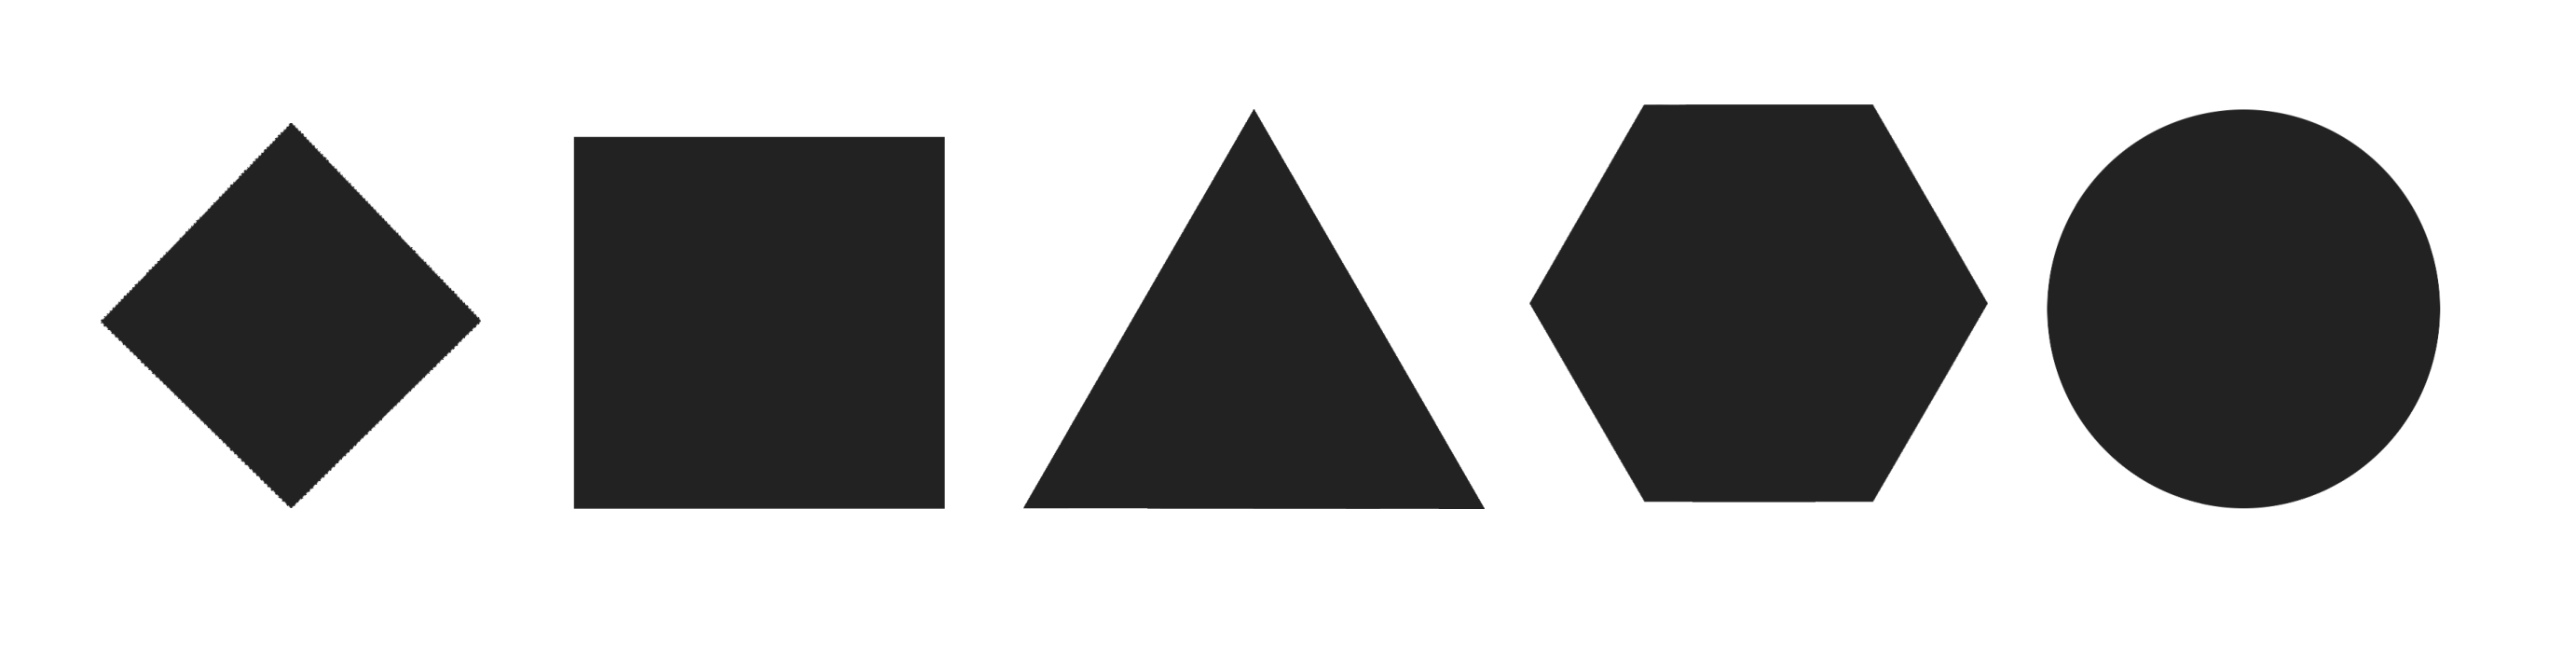
\includegraphics[scale=0.15]{figures/experiment_2_stimuli.pdf}
  \end{center}
\end{figure}

Stimuli were common solid geometric shapes, shown in Figure \ref*{figure:exp2-stimuli}.
Common and rare category labels were turned into features X and Y respectively.
Each shape was randomly allocated to one of the abstract features shown in Table \ref*{tab:abstract-exp2}.

\subsubsection{Procedure}

\begin{table}[!ht]
  \begin{center}
    \caption{Abstract design of Experiment 2 including both test and training phases. X and Y are in place of the category labels common and rare. During the test phase, participants needed to select either X or Y to complete the features shown below.\\}
    \label{tab:abstract-exp2}
    \begin{tabular}{llr} % text alignments
      \textbf{Training (Relative Frequencies)} & \textbf{Test}& \\
      \hline
      % & \\
      ABX x 3 &  A, B, C,        & \\
      ACY x 1 &  AB, AC, BC      & x 20 \\
      \hline
    \end{tabular}
  \end{center}
\end{table}

Table \ref*{tab:abstract-exp2} depicts the abstract experiment design.
Similar to the previous experiment, participants completed two phases: an encoding/training and a test phase.
In the training/encoding phase, participants were repeatedly exposed to the exemplars and were asked to memorize the arrangement of geometric shapes.
Compared to Experiment 1, exemplars were composed of three geometric shapes.
On each trial, geometric shapes appeared in random order so the position of features on the screen was completely counterbalanced.
This resulted in 24 trials within each block, which contained 18 common trials and 6 rare trials.
Similar to Experiment 1, participants could complete a maximum of 5 blocks.
After the first block, they were given a chance after completing each block to move straight to the test phase.
The trial structure and response deadlines corresponded to Experiment 1.

In the test phase, participants were shown \textit{incomplete} arrangements of geometric shapes and were asked to complete them.
On each test trial, they were asked to select either \textbf{X} or \textbf{Y} to complete the arrangement.
Similar to Experiment 1, each test item (incomplete arrangement of shapes) appeared 20 times.
Various arrangement of shapes appeared in the middle of the screen.
The response options X and Y with the corresponding shapes were shown below.
The prompt asked participants to pick one of the shapes to complete the arrangement.
Participants could respond by pressing either X or Y on the keyboard.
The test phase was composed of 120 trials presented across 5 blocks of 24 trials.
\\

\subsubsection{Analysis and Exclusion}

We applied the same analysis and exclusion methods as in Experiment 1.

\subsection{Results and Discussion}

After exclusion, 86 participants made it into our analysis.
The group-level mean probabilities are shown in Table \ref{tab:results-exp2}.
The results are a qualitative and ordinal match to Experiment 1.
Participants showed a clear common preference for stimuli A, $M_{A} = 0.78$, 95\% HDI $[0.73, 0.83]$, $\mathrm{BF}_{10} = 5.37 \times 10^{13}$.

\begin{table}[H]
  \begin{center}
    \caption{Group-level mean probabilities for each stimulus presented during the test phase in Experiment 2 after exclusion.\\}
    \label{tab:results-exp2}
    \vskip 0.12in
    \begin{tabular}{rcc}
      \hline
       & $P(common)$ & $P(rare)$ \\
       \hline
      A & 0.78 & 0.22\\
      AB & 0.95 & 0.05\\
      AC & 0.08 & 0.92\\
      B & 0.92 & 0.08\\
      \textbf{BC} & \textbf{0.27} & \textbf{0.73}\\
      C & 0.07 & 0.93\\
    \end{tabular}
  \end{center}
\end{table}

Participants also showed a reliable rare preference on ambiguous BC trials, $M_{BC} = 0.73$, 95\% HDI $[0.67, 0.79]$, $\mathrm{BF}_{10} = 8.12 \times 10^{8}$.
This gives us a sufficient amount of evidence to conclude that we have observed the IBRE.

Here, we further demonstrated that the IBRE can arise without experimental-design components that explicitly promote an error-driven process.

\section{Discussion}

In this study, we tested a central assumption of the most prominent theories of the IBRE.
This central assumption was that the IBRE is caused by the presence of prediction error.

In our first experiment, we implemented an observational learning version of the canonical IBRE procedure.
This meant that features and category labels appeared on the screen at the same time.
Participants learned about categories by reading complete sentences that described what symptoms people exhibited and what diseases they had.
The experiment included no feedback and required no responses from participants during training.
From a theoretical perspective, there was no opportunity for making an explicit error.
Nevertheless, we observed the inverse base-rate effect.
One limitation of this approach was that there are assumed causal relationships between features (symptoms) and labels (diseases).
These relationships might predispose participants to make feature-to-label predictions, which could result in prediction error and attentional reallocation.

In our second experiment, we further removed the causal relationship between features and labels by changing the stimuli and their presentation.
Here, participants saw nothing but an arrangement of geometric shapes, where previous category labels were treated as features.
There were no causal links between features and labels.
When participants were asked to complete incomplete arrangements of these shapes, they still exhibited a rare bias on $BC$ trials.
We still observed the IBRE.

The two experiments together suggest that the necessary conditions to observe the IBRE are fewer than previously established.
In Experiment 2, the only remaining conditions are the two uniquely predictive features, an overlapping feature, sequential presentation and the base rate.
One hypothesized way asymmetric representation is manifested is the attentional tuning of cognitive representation of category exemplars.
This is not necessarily absent in our experiments but is not directly tested.
Our experiments do not give direct evidence against the role of attention in developing asymmetric representation or in its contributions to the emergence of the IBRE.
Nonetheless, it must not happen through an error-driven process as conceptualized in the most prominent theories of the IBRE.
To further investigate this, the cued-recall procedure could incorporate eye-tracking to measure dwell time and order of information encoding.
EXIT-like theories can informally predict longer fixations on $C$ relative to $B$ during training, but it is unclear what mechanism underlies this attentiontal allocation without an explicit error-driven process.
In addition, brain imaging could further elaborate on the overlap of activations between cued-recall and supervised learning procedures.
This would enable us to pinpoint the networks that uniquely underlie this rare preference but are independent of task demands.

In both our experiments, the IBRE occurred without any explicit detail in the experimental procedure that would result in prediction error.
Therefore, any theorized error-driven process must be able to operate without explicit feedback.
Most prominent theories and their corresponding formal specification rely on relocating attention in response to prediction error.
They are unable to accommodate the current experiments because they are not designed to encode information presented without feedback.
Our results suggest that there could be a secondary cause of the IBRE not captured by previous process models.

\subsection{Alternative Theories without Prediction Error}

There are alternative theories of the IBRE that do not rely on processes that calculate prediction error.
A version of the dissimilarity-similarity generalized context model \citeA<DGCM, >{stewart2007dissimilarity} modified by \citeA{o2018model} has been proposed as an explanation of the IBRE.
From the perspective of DGCM, the main processes behind the rare preference are a combination of attention, memory strength of exemplars and dissimilarity from exemplars (stored category representations).
$BC \to rare$ arises due to the combination of the following factors: the high salience of $C$ relative to $B$ and the impact of the dissimilarity of $BC$ to the most remembered common category exemplar on the decision process.
Nonetheless, the model can accommodate these results only informally because it does not specify the mechanisms which encode information and produce the attentional values of each stimulus.
DGCM is a model of the test phase.
In that sense, the current experimental manipulations cannot be represented in the model.
This is the same challenge we encountered with process models - the specifications of these theories are unable to incorporate the changes to the experimental procedure.

Another alternative explanation is an eliminative-inference model \cite<ELMO, >{juslin2001high}.
This approach considers the $BC \to rare$ bias to result from rule-learning and post-training inferential processes during $BC$ trials.
The process is most similar to \textit{strategic guessing} \cite{kruschke1995extensions}.
Because of the dissimilarity of $BC$ to the most frequently applied rule, $B \to common$, participants use the most similar rule applicable to $BC$ from a "guessing set", $C \to rare$.
This results in the $BC \to rare$ bias.
Informally, ELMO could accommodate the observational learning paradigm, because of the presence of feature-to-label causality.
Participants could extract the same rules hypothesised to underlie the rare bias in the standard procedure.
Due to this presumed causality, ELMO could hypothesise that people encode rules about symptoms and diseases, which will similarly result in $BC \to rare$ during test.
But it is unclear how it could deal with the cued-recall implementation, as there is no clear-cut feature-to-label relationship in the stimuli presentation that drives rule formation.
In addition, ELMO also predicts the IBRE in the absence of a shared cue, even though humans do not show the IBRE under those conditions \cite{kruschke2001inverse}.
% One possibility is to assume that rules are formed between features only, but ELMO is not designed to deal with between-feature relationships.

\section{Conclusion}

Across two experiments, we investigated whether the demonstration of the IBRE requires the prediction-and-feedback components of the standard experimental procedure.
In Experiment 1, we conducted a successful conceptual replication of \citeA{johansen2007paradoxical}, which gave evidence for the IBRE being independent of supervised learning procedures.
In addition, Experiment 2 further suggests that the IBRE generalizes beyond simple predictive-learning \cite<e.g. >{medin1988problem,kruschke1996base,wills2014attention} and decision-making \cite{johansen2007paradoxical} paradigms.
This further suggests prediction error in terms of explicit feedback is not a necessary condition.
Theories of IBRE are inadequate to account for these findings, largely because of their inability to extend beyond supervised learning.

\section{Open Science}

We have made available the two experiments written in javascript, the analysis code, the raw data, and all other supplementary materials.
Experiment 1 is shared via \href{https://osf.io/auwvt/}{https://osf.io/auwvt/}, and \href{https://github.com/lenarddome/ply216-observational-ibre}{https://github.com/lenarddome/ply216-observational-ibre}.
Experiment 2 is shared via \href{https://osf.io/2tmc4/}{https://osf.io/2tmc4/} and \href{https://github.com/lenarddome/ply222-non-causal-ibreBA}{https://github.com/lenarddome/ply222-non-causal-ibre}.
The main repository that includes this manuscript and links to the materials for the two experiments can be found on \href{https://github.com/lenarddome/pu093-errorless-attentionless-ibre}{https://github.com/lenarddome/pu093-errorless-attentionless-ibre}.

\section{Acknowledgement}

The data for Experiment 1 was collected as part of a final-year undergraduate project. We thank for the help and contributions of Selena Lockett and Charlotte Hubbard in the data collection for Experiment 1.

\bibliographystyle{apacite}

\setlength{\bibleftmargin}{.125in}
\setlength{\bibindent}{-\bibleftmargin}

\bibliography{library}

\end{document}
